\chapter{Métricas de Software}
\label{chap:metricas}

\section{Processo de Medição}

Segundo o \cite{Guiaimplementacao} o processo Medição é um processo que apoia os processos de gerência e melhoria de processo e de produto, sendo um dos processos principais para gerenciar as atividades do ciclo de vida do trabalho e avaliar a viabilidade dos planos de trabalho. O propósito da Medição é coletar e analisar os dados relativos aos produtos desenvolvidos e aos processos implementados na organização e em seus trabalhos, de forma a apoiar o efetivo gerenciamento dos processos e demonstrar objetivamente a qualidade dos produtos\cite{ISO:12207}.

Ainda segundo o \cite{Guiaimplementacao} Entende-se por método de medição uma sequência lógica de operações, descritas genericamente, usadas para quantificar um atributo com respeito a uma escala especificada. Esta escala pode ser nominal, ordinal ou de razão (de proporção), bem como definida em um intervalo. 

\begin{easylist}[itemize]	
	
	& \textbf{Nominal:} A ordem não possui significado na interpretação dos valores \cite{Meirelles2013}
	& \textbf{Ordinal:} A ordem dos valores possui significado, porém a distância entre os valores não. \cite{Meirelles2013}
	& \textbf{Intervalo:}  A ordem dos valores possui significado e a distância entre os valores também. Porém, a proporção entre os valores não necessariamente possui significado. \cite{Meirelles2013}
	& \textbf{Racional:} Semelhante a a medida com escala do tipo intervalo, porém a proporção possui significado. \cite{Meirelles2013}

	\end{easylist}

	
	A \citeonline{ISO:15939} também divide o processo de medição em dois métodos diferentes, que se distinguem pela natureza do que é quantificado:
	
	\begin{easylist}[itemize]

	& \textbf{Subjetiva:} Quantificação envolvendo julgamento de um humano
	& \textbf{Objetiva:} Quantificação baseada em regras numéricas. Essas regras podem ser implementadas por um humano.

	\end{easylist}


%---------------------------------------------------------------------------------------------------------------------%

\section{Definição das métricas de software}

As métricas de software são medidas resultantes da medição do produto ou do processo do \textit{software} pelo qual é desenvolvido, sendo que o produto de \textit{software} deve ser visto como um objeto abstrato que se desenvolveu a partir de uma declaração inicial da necessidade de um sistema para um software finalizado, incluindo o código-fonte e as várias formas de documentação produzida durante o desenvolvimento \citeonline{Mills:1999}. Estas medidas resultantes podem ser estudas para serem utilizadas para medir a produtividade e a qualidade do produto. 


\cite{Mills:1999} classifica as métricas de software como métricas de produtos ou métricas de processo, essa divisão pode ser vista na figura \ref{modelodequalidade}. 

\begin{easylist}[itemize]	

& \textbf{Métricas de produtos:} são as medidas do produto de software em qualquer fase do seu desenvolvimento, a partir dos requisitos do sistema. Métricas de produto podem medir a complexidade da arquitetura do software, o tamanho do programa(código-fonte), ou o número de páginas de documentos produzidos. 

& \textbf{Métricas de processo:} são as medidas do processo de desenvolvimento de software, como o tempo de desenvolvimento global, o tipo de metodologia utilizada, ou o nível médio da experiência da equipe de programação.

\end{easylist}

\begin{figure}[h!]
\centering
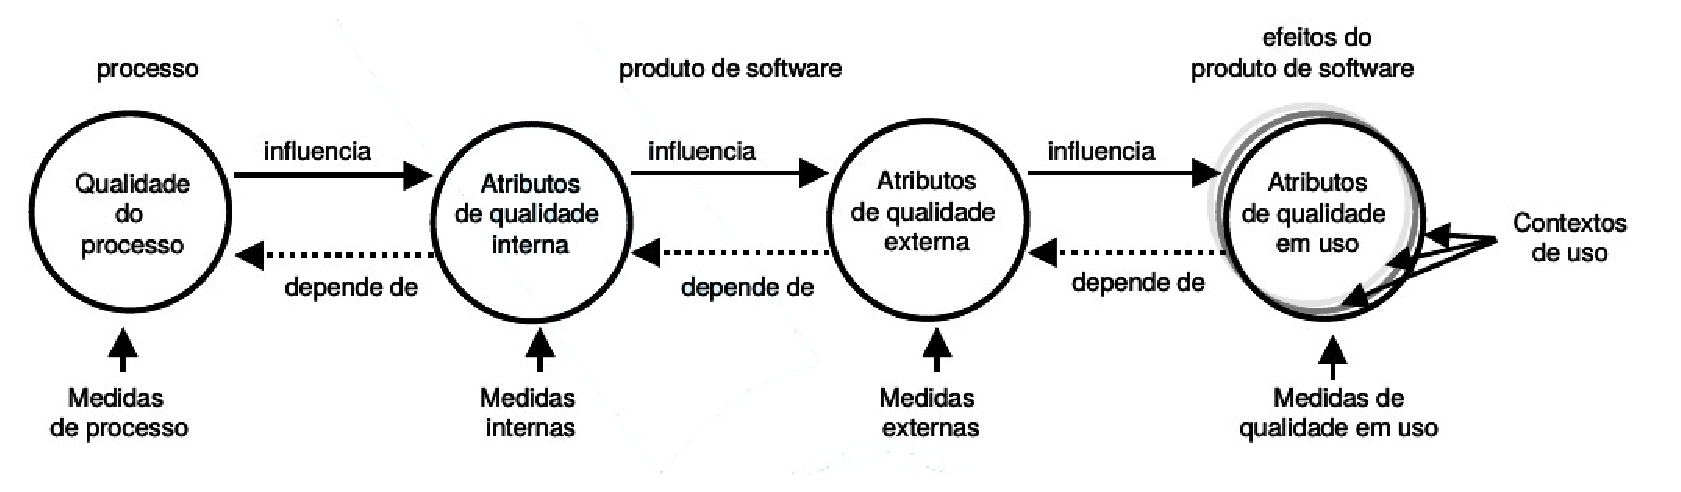
\includegraphics[keepaspectratio=false,scale=0.65]{figuras/figuras_nilton/modeloqualidade.eps}
\caption{Modelo de Qualidade do Produto da \citeonline{ISO:9126}}
\label{modelodequalidade}
\end{figure}
\FloatBarrier

A figura \ref{modelodequalidade} também pode ser notado a classificação das métricas de acordo com os diferentes tipos de medição, refletindo como as métricas influenciam nos contextos em que elas estão envolvidas, A qualidade do produto de software pode ser avaliada medindo-se os atributos internos (tipicamente medidas estáticas de produtos intermediários), os atributos externos (tipicamente pela medição do comportamento do código quando executado) ou os atributos de qualidade em uso \cite{ISO:9126}.

\begin{easylist}[itemize]

 & \textbf{Métricas internas:} Aplicadas em um produto de software não executável, como código fonte. Oferecem aos usuários, desenvolvedores ou avaliadores o benefício de poder avaliar a qualidade do produto antes que ele seja executável.
& \textbf{Métricas externas:} Aplicadas a um produto de software executável, medindo o comportamento do sistema do qual o software é uma parte através de teste, operação ou mesmo obervação. Oferecem aos usuários, desenvolvedores ou avaliadores o benefício de poder avaliar a qualidade do produto durante seu processo de teste ou operação.
& \textbf{Métricas de qualidade em uso:} Aplicadas para medir o quanto um produto atende as necessidades de um usuário para que sejam atingidas metas especificadas como eficácia, produtividade, segurança e satisfação.

\end{easylist}


%---------------------------------------------------------------------------------------------------------------------%

\section{Métricas de código fonte}

A definição de código-fonte segundo a SCAM é qualquer descrição executável de um sistema de software sendo incluído código de máquina, linguagens de alto nível e por representações gráficas executáveis \cite{harman}.

Segundo \cite{Mills:1999} a maior parte do trabalho inicial em métricas de produto analisaram as características do código-fonte. A partir da experiência com métricas e modelos, tornou-se cada vez mais evidente que as informações de métricas obtidas anteriormente do ciclo de desenvolvimento pode ser de grande valor no controle do processo e dos resultados, o que sucedeu uma série de trabalhos tratando sobre o tamanho ou complexidade do software. 

Neste capítulo será evidenciado em duas categorias as métricas de código-fonte que serão utilizadas neste trabalho de conclusão de curso, métricas de tamanho e complexidade e métricas de orientação a objetos. Estas métricas são objetivas e serão calculadas a partir da análise estática do código-fonte de um software. 

%--------------------------------------------
\subsection{Métricas de tamanho e complexidade}

Cada produto do desenvolvimento de software é uma entidade física, como tal, pode ser descrito em termos de tamanho. Desde outros objetos físicos são facilmente mensuráveis (em comprimento, volume, massa, ou outra medida padrão), medir o tamanho do software deve ser relativamente simples e coerente de acordo com os princípios da teoria da medição. No entanto, na prática, a medição de tamanho apresenta grandes dificuldades\cite{Fenton98}. 

Segundo \cite{honglei_research_2009} as métricas de complexidade \textit{software} pertencem as principais medições de software e é o principal método para assegurar a qualidade do \textit{software}. Quanto menor a complexidade dos programas, melhor eles são, as métricas de complexidade também podem ser usadas para prever os defeitos ou erros. A seguir são apresentadas algumas métricas de tamanho e complexidade.

\begin{easylist}[itemize]

	& \textbf{LOC} (\textit{Lines of Code}): Métrica simples em que são contadas as linhas executáveis de um código, desconsiderando linhas em branco e comentários.  \cite{metricsandmodels} 
		
	& \textbf{ACCM} (\textit{Average Cyclomatic Complexity per Method}): Mede a complexidade do programa, podendo ser representada através de um grafo de fluxo de controle. \cite{McCabe76}

	& \textbf{AMLOC} (\textit{Average Method Lines of Code}): Indica a distribuição de código entre os métodos. Quanto maior o valor da métrica, mais pesado é o método. É preferível que haja muitos métodos com pequenas operações do que um método grande e de entendimento complexo. \cite{Meirelles2013}
	
\end{easylist}

\subsection{Métricas de Orientação a Objetos}

O surgimento da programação orientada a objetos representou uma importante mudança na estratégia de desenvolvimento, focalizando a atenção para conceitos mais próximos ao negócio modelado. \cite{phpmysql}  

Métricas de orientação a objetos foram adotadas devido à grande utilização desse paradigma no desenvolvimento de software. Serão adotadas as seguintes métricas já selecionadas por \citeonline{rego_monitoramento_2014}:  

\begin{easylist}
	
	%--------------------------
	& \textbf{ACC} (\textit{Afferent Connections per Class} - Conexões Aferentes por Classe): Mede a conectividade entre as classes. Quanto maior a conectividade entre elas, maior o potencial de impacto que uma alteração pode gerar. \cite{Meirelles2013}
	
	%--------------------------
	& \textbf{ANPM} (\textit{Average Number of Parameters per Method} - Média do Número de Parâmetros por Método): Indica a média de parâmetros que os métodos possuem. Um valor muito alto para quantidade de parâmetros pode indicar que o método está tendo mais de uma responsabilidade. \cite{Basili1987}

	%--------------------------
	& \textbf{CBO} (\textit{Coupling Between Objects} - Acoplamento entre Objetos): Essa é uma métrica que diz respeito a quantas outras classes dependem de uma classe. É a conta das classes às quais uma classe está acoplada. 		Duas classes estão acopladas quando métodos de uma delas utilizam métodos ou variáveis de outra. Altos 			valores dessa métrica aumentam a complexidade e diminuem a manutenibilidade.  \cite{softwaremeasurementandestimation}.
  		 
	%-----------------------------
	& \textbf{DIT} (\textit{Depth of Inheritance Tree} - Profundidade da 
	Árvore de Herança): Responsável por medir quantas camadas de herança compõem uma determinada hierarquia 		de classes \cite{softwaremeasurementandestimation}. Segundo \citeonline{Meirelles2013}, quanto maior o valor de DIT, maior o número de métodos e atributos herdados, portanto maior a complexidade.

	%--------------------------
	& \textbf{LCOM4} (\textit{Lack of Cohesion in Methods} - Falta de Coesão
	entre Métodos): A coesão de uma classe é indicada por quão próximas as variáveis locais estão relacionadas com variáveis de instância locais. Alta coesão indica uma boa subdivisão de classes. A LCOM mede a falta de coesão através dissimilaridade dos métodos de uma classe pelo emprego de variáveis de instância.\cite{metricsandmodels}. A métrica LCOM foi revista e passou a ser conhecida como LCOM4, sendo necessário para seu cálculo a construção de um gráfico não-orientado em que os nós são os atributos e métodos de uma classe. Para cada método deve haver uma aresta entre ele e outro método ou variável. O valor da LCOM4 é o número de componentes fracamente conectados a esse gráfico \cite{Meirelles2013}

	%--------------------------
	& \textbf{NOC} (\textit{Number of Children} - Número de Filhos): É o número de sucessores imediatos,  (portanto filhos) de uma classe. Segundo \citeonline{softwaremeasurementandestimation}, altos valores indicam que a abstração da super classe foi diluída e uma reorganização da arquitetura deve ser considerada.
	
	%-----------------------------
	& \textbf{NOM} (\textit{Number of Methods} - Número de Métodos): Indica a quantidade de métodos de uma classe, medindo seu tamanho. Classes com muitos métodos são mais difíceis de serem reutilizadas pois são propensas a serem menos coesas. \cite{Meirelles2013}  

	%-----------------------------
	& \textbf{NPA} (\textit{Number of Public Attributes} - Número de Atributos Públicos): Mede o encapsulamento de uma classe, através da medição dos atributos públicos. O número ideal para essa métrica é zero \cite{Meirelles2013}

	%-----------------------------
	& \textbf{RFC} (\textit{Response For a Class} - Respostas para uma Classe): \citeonline{metricsandmodels} define essa métrica como o número de métodos que podem ser executados em respostas a uma mensagem recebida por um objeto da classe.

\end{easylist}	

%---------------------------------------------------------------------------------------------------------------------%

\section{Configurações de qualidade para métricas de código fonte} 

Em sua tese de doutorado, \citeonline{Meirelles2013} buscou responder as seguintes questões de pesquisa:
\begin{easylist}[itemize]

	& \textbf{QP1 -} Métricas de código-fonte podem influir na atratividade de projetos de software livre? 
	& \textbf{QP1 -} Quais métricas devem ser controladas ao longo do tempo?		
	& \textbf{QP3 -} As métricas de código-fonte melhoram com o amadurecimento do projeto?	
	
\end{easylist}

Para responder essas questões, sua pesquisa concentrou-se em alguns objetivos tecnológicos e científicos, fazendo uso da técnica estatística descritiva percentil para identificação das distribuições dos valores de métricas em 38 projetos de software livre, observando os valores frequentes dessas métricas de modo a servirem de referência para projetos futuros. 

O percentil são pontos estimativos de uma distribuição de frequência que determinam a porcentagem de elementos que se encontram abaixo deles. Por exemplo, quando se diz que o valor 59,0 da métrica rfc do projeto \textbf{Open JDK8} está no percentil 90, significa dizer que 90\% dos valores identificados para essa métrica estão abaixo de 59,0. 

A tabela \ref{tab:percentil} abaixo pôde ser criada graças ao uso da técnica estatística citada:
	
	\begin{table}[!ht]
	\begin{center}
	
	\input{tabelas/tabelasMatheus/percentis.ltx} 
	\caption{Percentis para métrica RFC em projetos Java extraídos de  
	\citeonline{Meirelles2013}}
	\label{tab:percentil}
	\end{center}
	\end{table}	
	\FloatBarrier	

Através dos resultados obtidos para cada métrica, \citeonline{Meirelles2013} observou que era possível identificar valores frequentes analisando os percentis. Na \ref{tab:percentil}, por exemplo, foram observados no projeto \textbf{Open JDK8} valores de 0 a 9 como muito frequentes, de 10 a 26 como frequente, de 27 a 59 como pouco frequente e acima de 59, que representa apenas 10\% do código-fonte do projeto, como não frequente \cite{Meirelles2013}. A seguinte tabela foi extraída do trabalho de conclusão de curso de \citeonline{rego_monitoramento_2014} para que fosse criada uma relação entre o intervalo de frequência e o intervalo qualitativo de uma métrica, afim de facilitar sua interpretação:

\begin{table}[!ht]
	\begin{center}
	\input{tabelas/tabelasMatheus/intervalos.ltx}
	\caption{Nome dos Intervalos de Frequência extraídos de \citeonline{rego_monitoramento_2014}}
	\label{tab:nomes}
	\end{center}
	\end{table}
	\FloatBarrier
	
	 
\citeonline{Meirelles2013} destaca na avaliação dos resultados a maneira como o \textbf{Open JDK8} demonstrou um equilíbrio no valor das métricas em relação aos demais projetos Java, de modo que seus valores são frequentemente usados como referência na interpretação dos valores das métricas. Se de um lado o  \textbf{Open JDK8} demonstrou os menores valores percentis, os valores mais altos foram identificados no \textbf{Tomcat}. \citeonline{rego_monitoramento_2014} considerou então os dois cenários para que as referências de valores para as métricas fossem criadas. O resultado dessa análise gerou em seu trabalho a seguinte tabela:

\begin{table}[!ht]
	\begin{center}
	\input{tabelas/tabelasMatheus/metricas.ltx}	
	\caption{Configurações para os Intervalos das Métricas para Java extraídas de \citeonline{rego_monitoramento_2014}}
	\label{tab:good-metrics}
	\end{center}
	\end{table}
	\FloatBarrier
   

%---------------------------------------------------------------------------------------------------------------------%

\section{Cenários de limpeza} 
	